\section{Introduction}
I have spent the majority of my time this week struggling with Long - Short Term Memory network, seeking for applicable video classification methods and figuring out what made an image memorable.

\section{Video classification methods}
Matt Harvey's paper\cite{5videomethods} was about introducing some appropriate video classification methods. The author compared 5 different methods on UCF-101\cite{ucf101} to come up with the final results and his source code could be found \href{https://github.com/harvitronix/five-video-classification-methods}{here on his GitHub page}. Here was the summary of 5 video classification methods introduced by the author.

\textbf{\emph{Classify one frame at a time with a Convolutional Neural Network}}. Using this method meant we had ignored the temporal features of video and attempt to classify each video by looking at just a single frame. The most recommended technique for this method was using transfer learning to retrain a pre-trained Neural Network on different datasets such as ImageNet. We literally looked at each frame independently, and classified the entire video based solely on that one frame rather than looking at all the frames and doing any sort of averaging or max-ing. After training on UFC101, the author got the final test accuracy of ~65\% top 1.

\textbf{\emph{Use a time-distributed Convolutional Neural Network, passing the features to an Recurrent Neural Network, in one network}}. The author suggested first using the Kera's TimeDistributed wrapper distribute layers of Convolutional Neural Network across an extra dimension - time; secondly, forwarding this wrapper through our Recurrent Neural Network. This model must be trained from scratch. After training, the author got the final test accuracy of 20\%, which was much far from the baseline above. 

\textbf{\emph{Use a 3D Convolutional Neural Network}}. This seemed to be a reason-able method because 3D ConvsNet applied convolutions (and max pooling) in the 3D space, where the third dimension in our case was time. The author produced a network called C3D that achieved 52.8\% accuracy on UFC101. After training, the author got the final test accuracy of 28\%, which was also far from our baseline.

\textbf{\emph{Extract features with a Convolutional Neural Network, pass the sequence to a separate Recurrent Neural Network}}. First, we ran every frame from every video through Inception (or some other networks), saving the output from the final pool layer of the network (feature). So we effectively chop off the top classification part of the network so that we ended up with a 2,048-d vector of features that we couls pass to our RNN. Second, we converted those extracted features into sequences of extracted features. The author stated the this model achieved better than the CNN-only results. The concretely accuracy number was 74\%, which was significantly higher than our baseline.

\textbf{\emph{Extract features from each frame with a Convolutional Network Network and pass the sequence to an Multi-Layer Perceptron}}. The author applied the same Convolutional Neural Network extraction process as in the previous method, but instead of sending each piece of the sequence to an Recurrent Neural Network, we would flatten the sequence and pass the new \textbf{\emph{[40, 2048]}} input vector into a fully connected network (a multilayer perceptron). After training, the author got the final test accuracy of 70\%, which was higher than our baseline but lower than the previous method.

\section{What makes an image memorable?}
\subsection{Introduction}
After getting stuck in trying to improve the accuracy of my network architec-ture, I started researching which factors made an image or video memorable. I found a relevant paper in CVPR 2011 about this article which was \textbf{\emph{What makes an image memorable?}}\cite{imagememorable}.

Among the many reasons why an image might be remembered by a viewer, the authors investigated first the following factors: color, simple image features, object statistics, object semantics, and scene semantics.

\subsection{Color and simple image features}
The authors proposed a figure that demonstrate the correlation between memorability and basic pixel statistics. Mean hue was weakly predictive of memory: as mean hue transitions from red to green to blue to purple, memo-rability tended to go down ($\rho$ = -0.16). This correlation might be due to blue and green outdoor landscapes being remembered less frequently than more warmly colored human faces and indoor scenes. Mean saturation and mean value, on the other hand exhibited even weaker correlations with memorability. 

\begin{figure}[!ht]
\centering
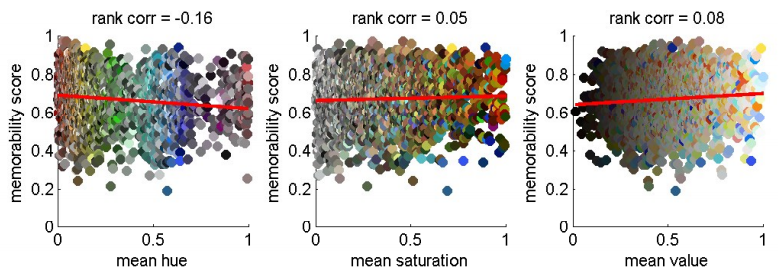
\includegraphics[width=\textwidth]{week10-color-simpe-features.png}
\caption{Correlation between Simple image features and Memorability.}
\end{figure}

These findings concorded with other work that had shown that perceptual features were not retained in long term visual memory\cite{simplefeatures}. In order to make useful predictions, more descriptive features were likely necessary.

\subsection{Object statistics}
Using LabelMe\cite{labelme}, each image in target set was segmented into object regions and each of these segments was given an object class label by a human user (e.g “person,” “mountain,” “stethoscope”). In this section, the authors quantified the degree to which the data could be explained by non-semantic object statistics. The authors found that none of these statistics above made good predictions on their own. 

\begin{figure}[!ht]
\centering
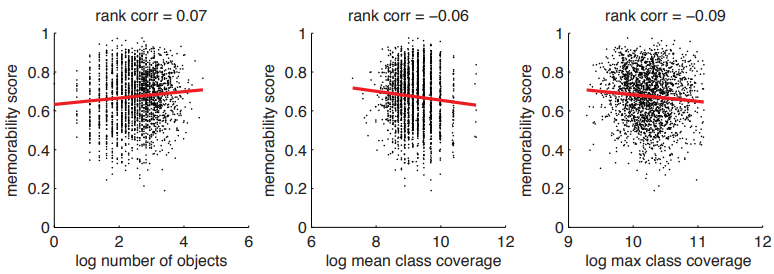
\includegraphics[width=\textwidth]{week10-object-statistics.png}
\caption{Correlation between Simple Object Statistics and Memorability 1.}
\end{figure}
    
Simple object statistics (log number of objects, log mean pixel coverage over present object classes, and log max pixel coverage over object classes) did not correlate strongly with memorability ($\rho$ = 0.07, -0.06, and -0.09 respectively).

Beside that the authors also marginalized across classes to generate histo-grams of Object Counts, Object Areas and Multiscale Object Areas. And these factors' correlation were even smaller than those of the color and simple image features.

\begin{figure}[!ht]
\centering
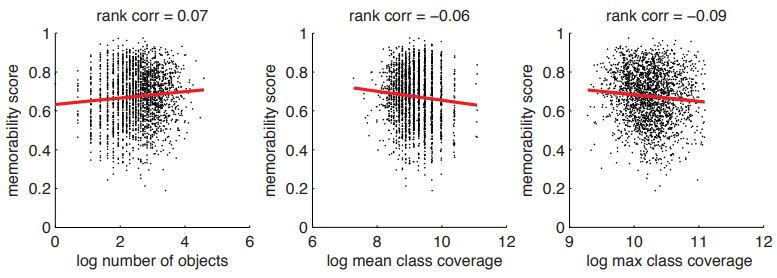
\includegraphics[width=\textwidth]{week10-image-class.png}
\caption{Correlation between Simple Object Statistics and Memorability 2.}
\end{figure}

\subsection{Object and scene semantics}
As demonstrated above, objects without semantics were not effective at predicting memorability. Using regression on the entire joint (object class, statistic), the authors proposed a comparision table of predicted versus mea-sured memorabilities.

\newpage
\begin{figure}[!ht]
\centering
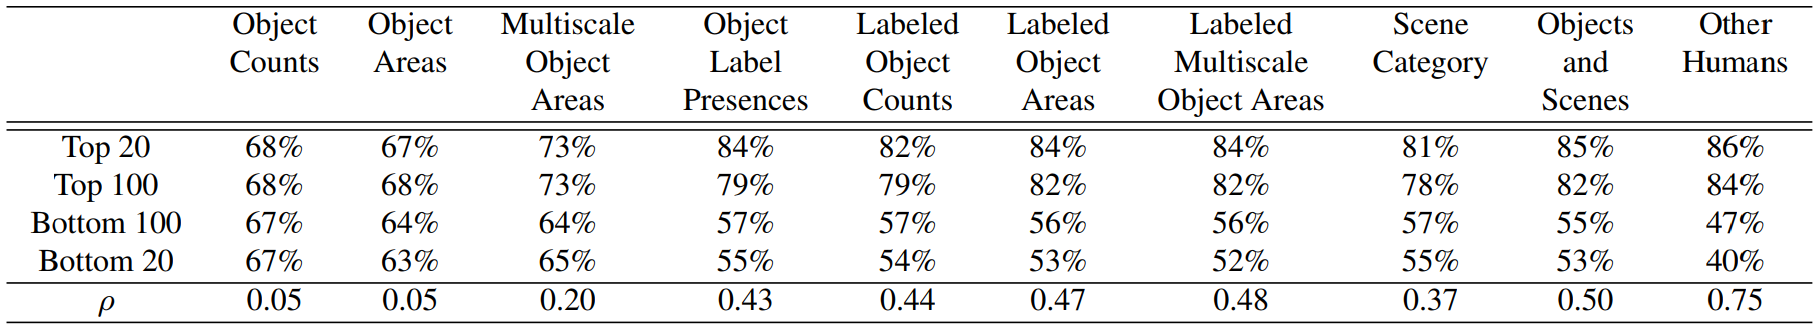
\includegraphics[width=\textwidth]{week10-prediction-comparision}
\caption{Comparision of Predicted versus Measured Memorabilities.}
\end{figure}

Even the Object Label Presences alone, which simply convey a set of se-mantic labels and otherwise did not describe anything about the pixels in an image, performed well above the authors' best unlabeled object statistic, Multiscale Object Areas ($\rho$ = 0.43 and 0.20 respectively). Moreover, Scene Category, which just gave a single label per image, appeared to summarize much of what makes an image memorable ($\rho$ = 0.37), and the best method was to combine both object and scene semantic information ($\rho$ = 0.50). These performances supported the idea that object and scene semantics were a primary substrate of memorability.

\subsection{Visualizing what makes an image memorable}
Since object content appears to be important in determining whether or not an image would be remembered, the authors further investigated the contri-bution of objects by visualizing object-based memory maps for each image.

This visualization gave a sense of how objects contribute
to the memorability of particular images. The authors additionally interested in which objects were important across all images so they estimated an object’s overall contribution as its contribution per image, calculated as above, averaged across all test set images in which it appeared with substantial size. The authors sorted objects into an intuitive ordering: people, interiors, foregrounds, and human-scale objects tend to contribute positively to memorability; exteriors, wide angle vistas, backgrounds, and natural scenes tend to contribute negatively to memorability.

\begin{figure}[!ht]
\centering
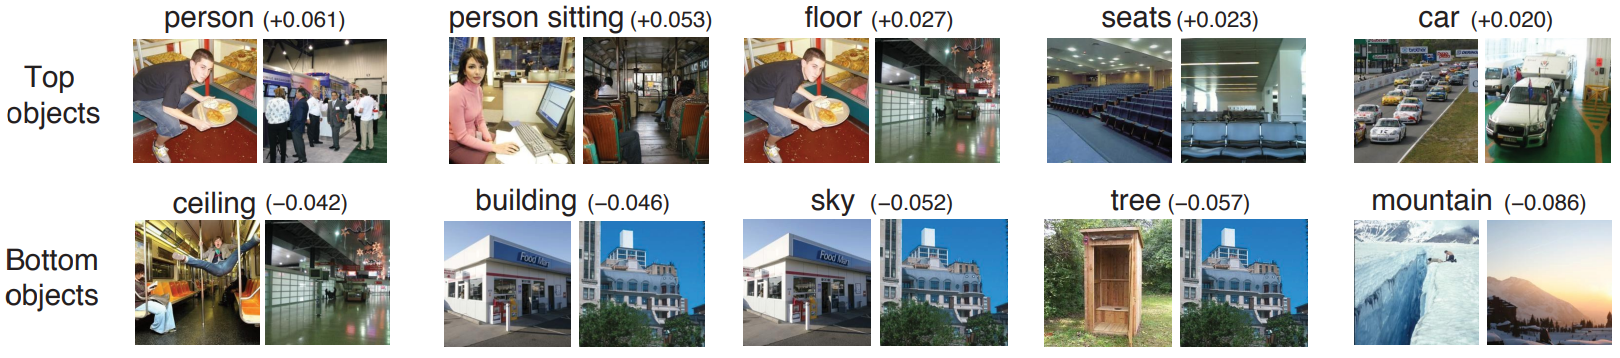
\includegraphics[width=\textwidth]{week10-object-impact.png}
\caption{Objects sorted by their predicted impact on memorability.}
\end{figure}

\newpage
\begin{figure}[!ht]
\centering
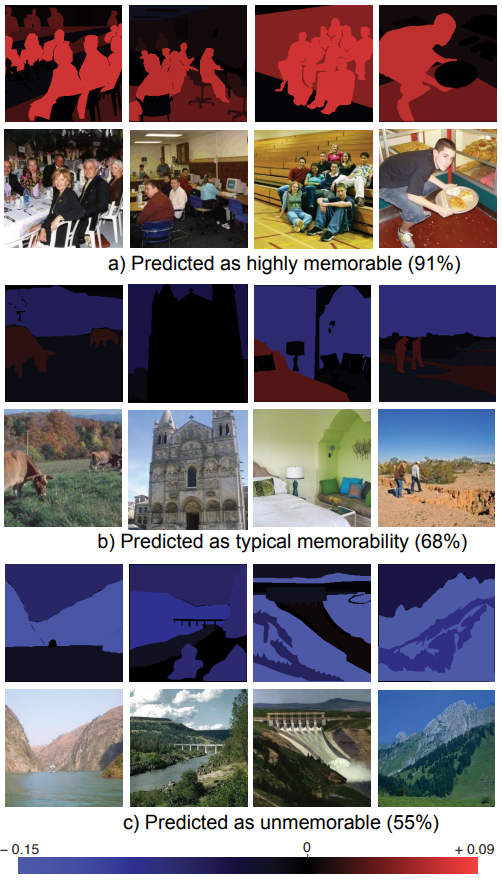
\includegraphics[width=0.8\textwidth]{week10-object-contribution.png}
\caption{Visualization of how each object contributes to the memorability of sample images spanning a range of memorability predictions. In red were objects that contribute to higher predicted memorability and in blue were objects that contribute to lower predicted memorability. Brightness was proportional to the magnitude of the contribution.}
\end{figure}


\section{PyTorch LSTM Classification Network}
\subsection{Architecture}
I misunderstood between the concept of number of layers and number of Long - Short Term Memory (LSTM) cells so the training time was nearly 4 times longer than normal. For more details, the number of LSTM cells that PyTorch used was actually the quantity of sequences we feed into the LSTM network at once. So in my case it was 8 (because each video had 8 frames, and I feed all 8 frames once). The number of layers term in PyTorch meant how many times I wanted to stack the 8-LSTM-cell sequence to form a  \textbf{\emph{8 \( \times \) num\_layers}} grid of LSTM cells.

Each LSTM cell had multiple LSTM units, and the quantity of units was defined by \textbf{\emph{hidden\_size}} parameter. The figure below described correctly the Long - Short Term Memory model architecture in PyTorch.

\begin{figure}[!ht]
\centering
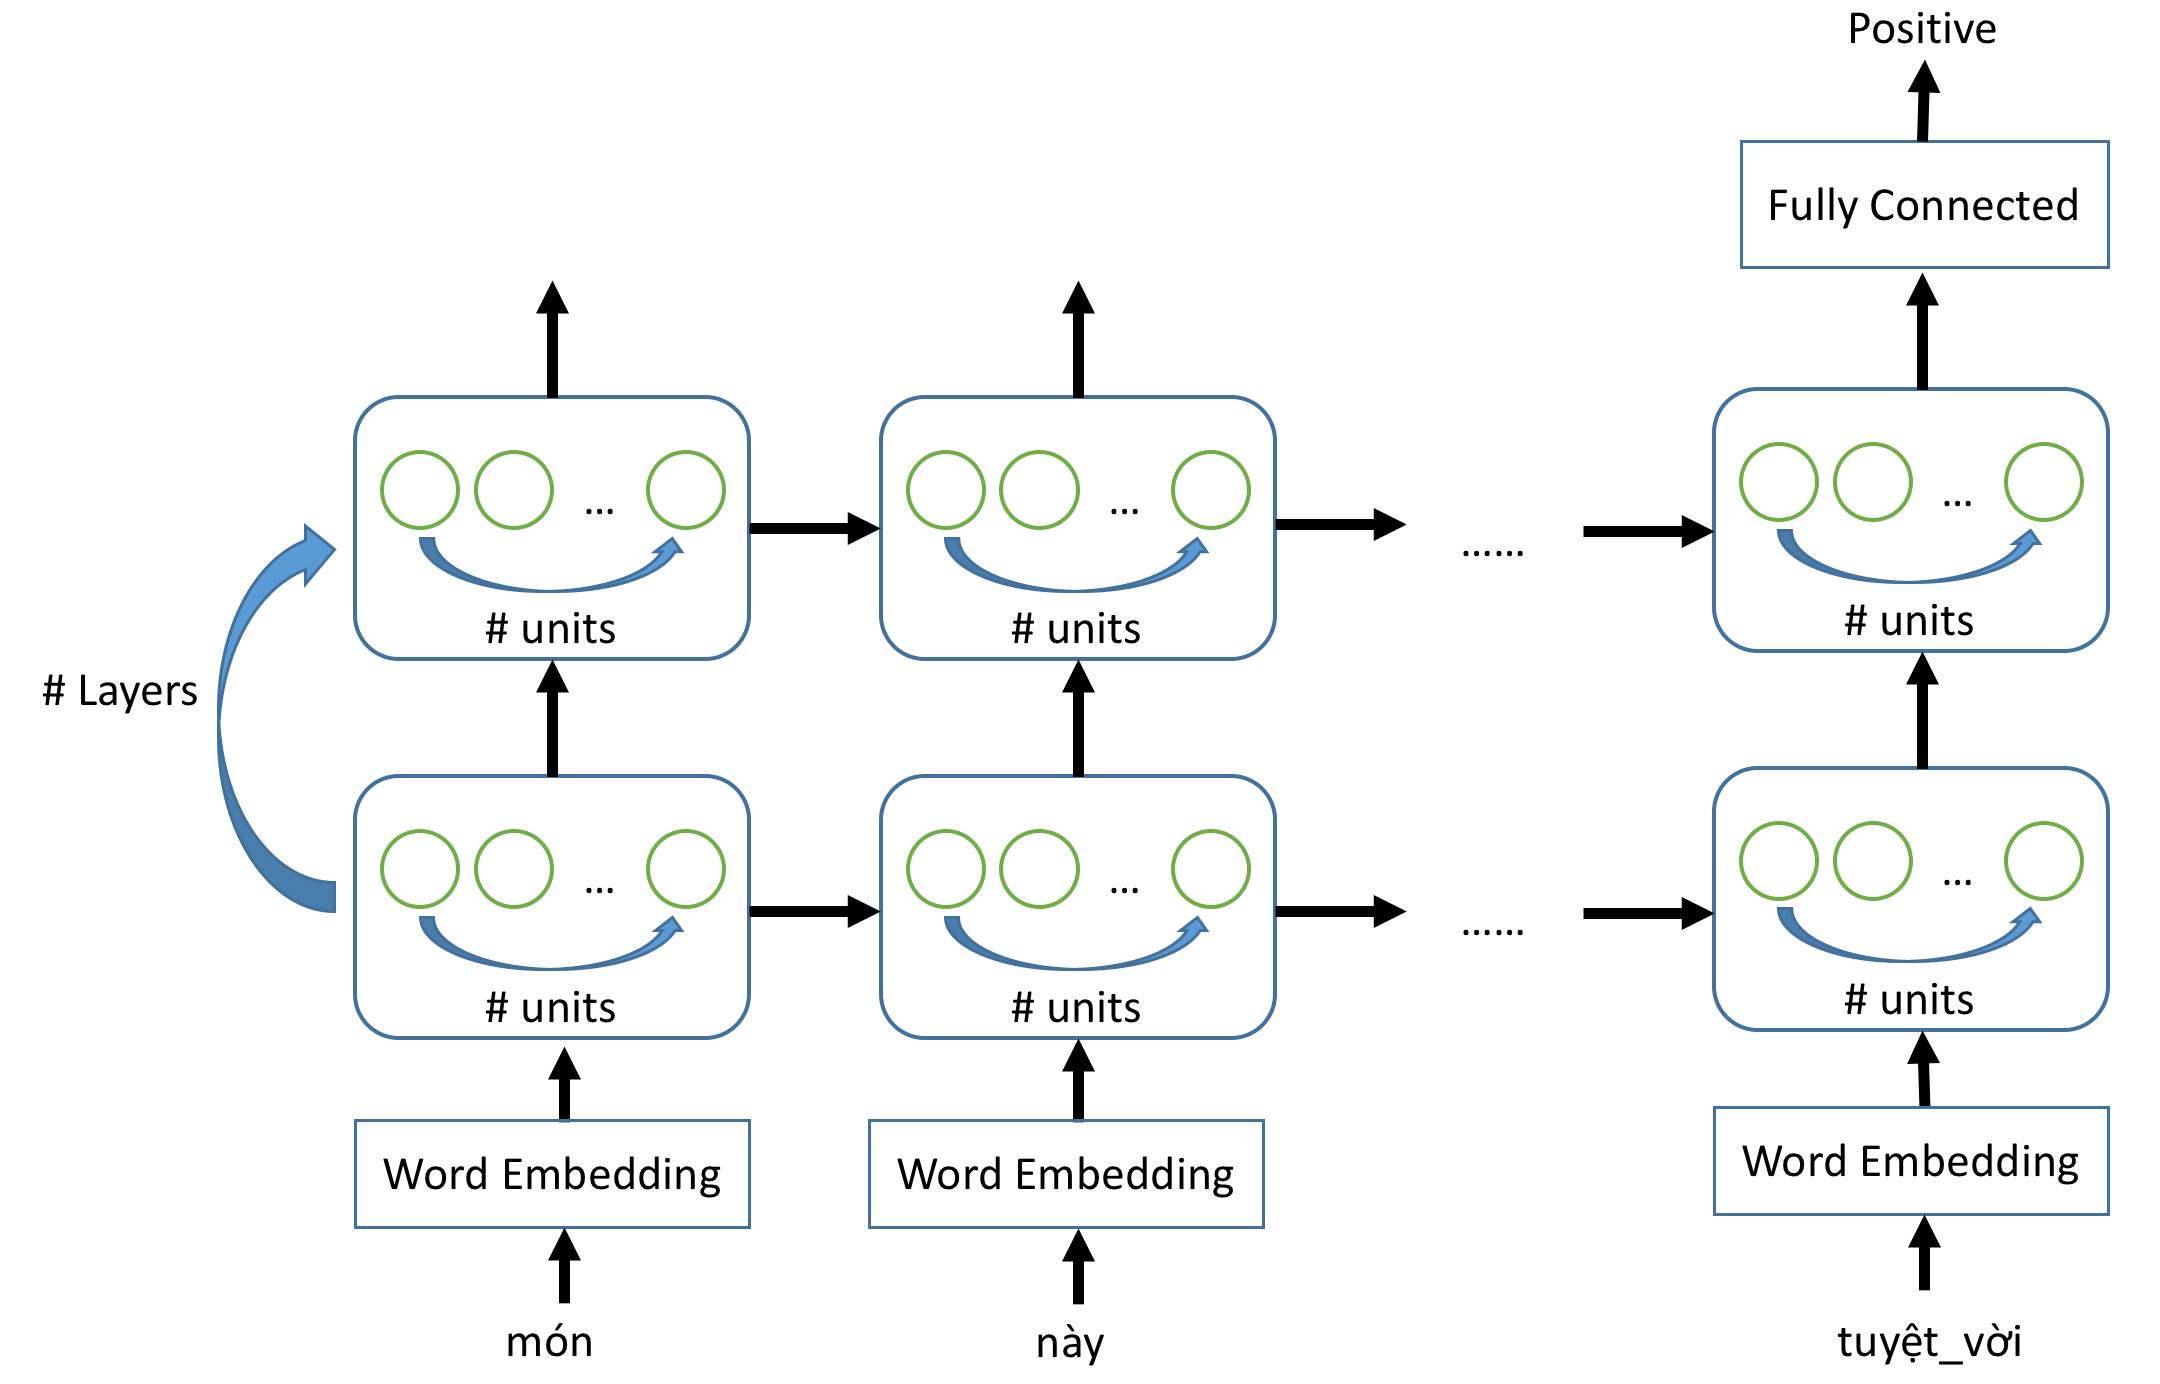
\includegraphics[width=\textwidth]{week10-lstm-architecture.png}
\caption{Long - Short Term Memory Network Architecture.}
\end{figure}

The smallest unit in the network above was the LSTM unit, multiple LSTM units formed one LSTM cell, each cell took responsibility for one input feature (multiple input features formed the input sequence). Multiple LSTM cells formed one LSTM layer. Stacking multiple LSTM layers formed one Stacked LSTM network.

\subsection{Training on Dev-Set (extracted by ResNet50)}
\subsubsection{Strategy}
The purpose of this challenge was to calculate the memorability score for each video, and this calculation was so ambiguous so I broke this problem into the classification problem of \textbf{\emph{11}} categories. So after getting the classify results, I would devide them by 10 to get numbers which were similar to the scores required by the challenge. My strategy was to splitted the provided dev-set for this challenge into two parts, since the dev-set had 8000 videos, I picked \textbf{\emph{6000}} videos for training and \textbf{\emph{2000}} for testing.

\subsubsection{Version 1}
My network architecture contained 2 parts; the first part was the Long - Short Term Memory part, took the sequence of input and gave a sequence of output; the second part was the Fully-connected layer acted as the classifier. I used a sequence of 8 LSTM cells took in input of size \emph{[8, 2048]} and lately produced output of size \textbf{\emph{[8, 8]}}. Next, I flattened that array and passed it through the Fully-connected Layer to finally got the classification score for \emph{11} classes. There was a figure below to demonstrate exactly how my architecture was.

I trained this architecture with \textbf{\emph{200}} epochs and at the learning rate of \textbf{\emph{1e-1}}. But the result was not impressive to me at all. I think because the learning rate was too high for this kind of network. The loss and accuracy were completely turbulent over time.

The maximum accuracy was \textbf{\emph{26\%}} and the minimum value of loss was \textbf{\emph{74}} but those values were not reliable.

This architecture took me \textbf{\emph{3 hours}} to train 200 epochs (\textbf{\emph{54s}} per epoch).

\begin{figure}[!ht]
\centering
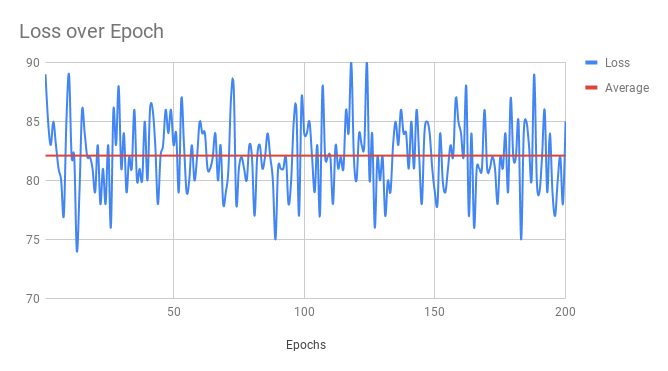
\includegraphics[width=\textwidth]{week10-devset-v1-loss.png}
\caption{Loss over Epoch.}
\end{figure}

\newpage
\begin{figure}[!ht]
\centering
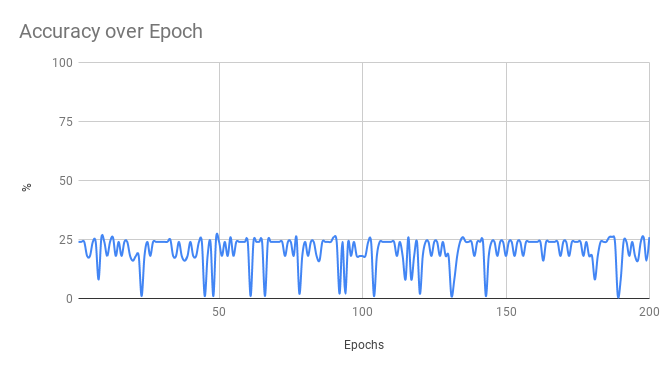
\includegraphics[width=\textwidth]{week10-devset-v1-accuracy.png}
\caption{Accuracy over Epoch.}
\end{figure}

\begin{figure}[!ht]
\centering
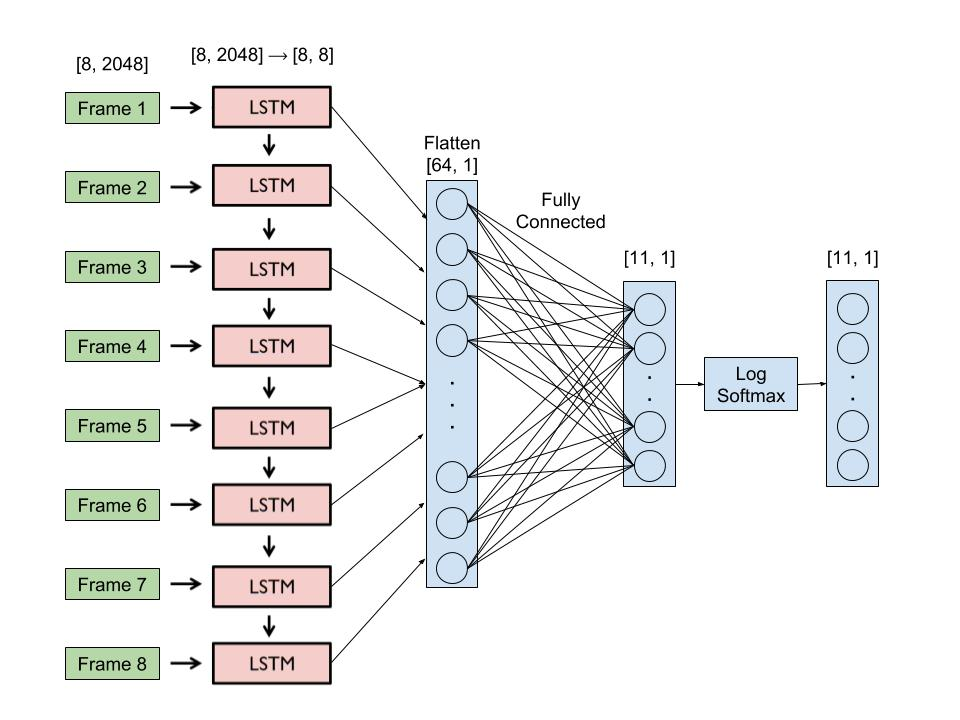
\includegraphics[width=\textwidth]{week10-lstmclassification-v1.jpg}
\caption{LSTM Classification v1.}
\end{figure}

\newpage
\subsubsection{Version 2}
I had edited some parameter of my network architecture and change the the learning rate as well as the number of epochs. I changed the output size of Long - Short Term Memory cells from \emph{[8, 8]} to \textbf{\emph{[8, 1024]}} to determine whether I would have better results or not. I also decreased the learning rate to \textbf{\emph{1e-5}} and the number of epochs to \textbf{\emph{90}} (the number of epochs was actually 100 but I got my Colab session shut down and the loss was 0 anyway so I kept that number at 90).

\begin{figure}[!ht]
\centering
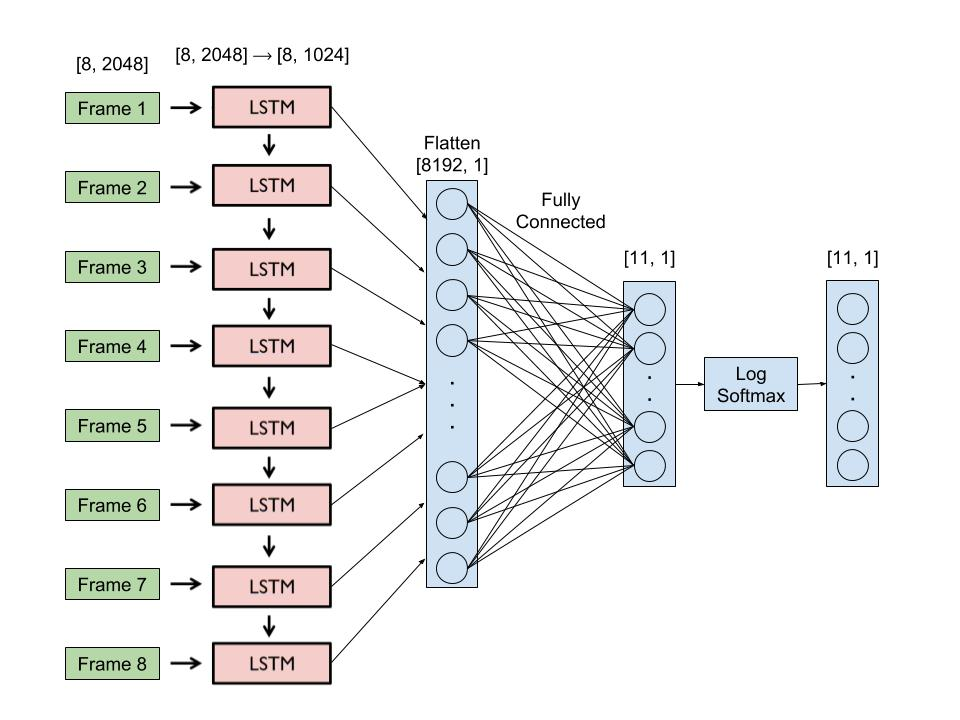
\includegraphics[width=\textwidth]{week10-lstmclassification-v2.jpg}
\caption{LSTM Classification v2.}
\end{figure}

I did not understand why after modifying the parameter of the network and learning rate, the initial loss value was drop from 89 to 1.8. The loss value was dropping over time as I expected, but unfortunately the accuracy was dropping too. At the time I got my loss value of 0, my test accuracy was just \textbf{\emph{21.6\%}}. The maximum accuracy was also \textbf{\emph{26\%}} and the minimum value of loss was \textbf{\emph{0}} but those values were not reliable. These figures below described the loss value and accuracy over epoch.

This architecture took me around \textbf{\emph{2 hours}} to train 90 epochs (\textbf{\emph{1.3 mins}} per epoch).

\newpage
\begin{figure}[!ht]
\centering
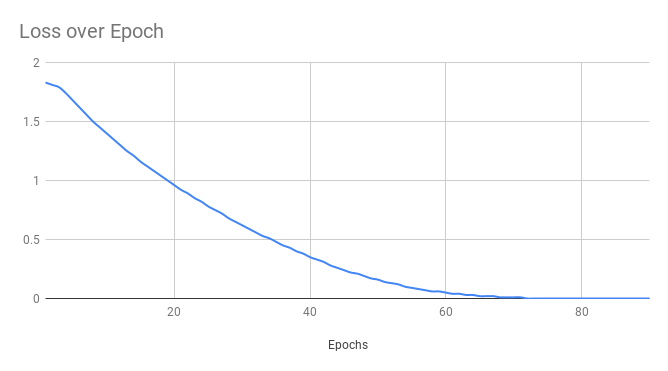
\includegraphics[width=\textwidth]{week10-devset-v2-loss.png}
\caption{Loss over Epoch.}
\end{figure}

\begin{figure}[!ht]
\centering
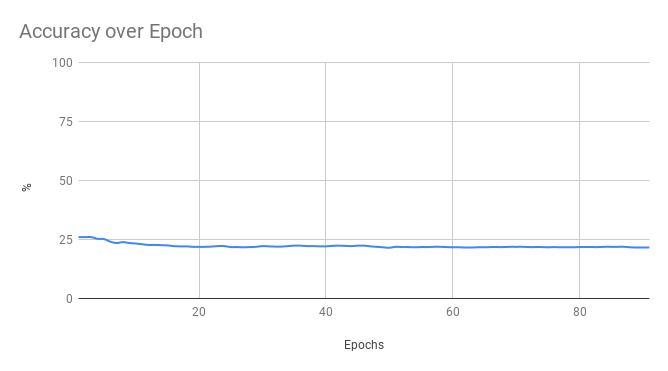
\includegraphics[width=\textwidth]{week10-devset-v2-accuracy.png}
\caption{Accuracy over Epoch.}
\end{figure}

\newpage
\subsection{Training on LaMem-Set (extracted by Inceptionv3)}
\subsubsection{Introduction}
Large - scale Image Memorability\cite{lamem} was a dataset from MIT containing original 60000 images from diverse sources and corresponding memorability scores for memorability predicting purpose. The authors also introduced a Convolutional Neural Network with fine - tuned deep features that outperformed all other features by a large margin, reaching a rank correlation of 0.64, near human consistency (0.68). The authors could generate a memorability maps (likely Class Activation Map) for each image by using the analysis of the res-ponses of the high - level CNN layers to shown which objects and regions were positively, and negatively, correlated with memorability.

\subsubsection{Strategy}
I used the same architecture as the Dev-set version v2 above to test this dataset. As the dataset had 55000 images when I downloaded it, I splitted this dataset into two parts, 45000 images for training and 10000 images for testing. I also have to change the number of Long - Short Term Memory cells in my network architecture to 1 because I had only one image at a time. I used Tensorflow's pre-trained Inceptionv3 convolutional neural network to convert those images above into feature vectors and then used them as the input of my network. 

\subsubsection{Version 1}
I used the learning rate of \textbf{\emph{1e-5}} and the number of epochs of \textbf{\emph{20}} (it was a small number because this dataset was huge and took so much time to deal with, and my purpose was just to test my network architecture). This figure below demonstrated how my network architecture was.

\begin{figure}[!ht]
\centering
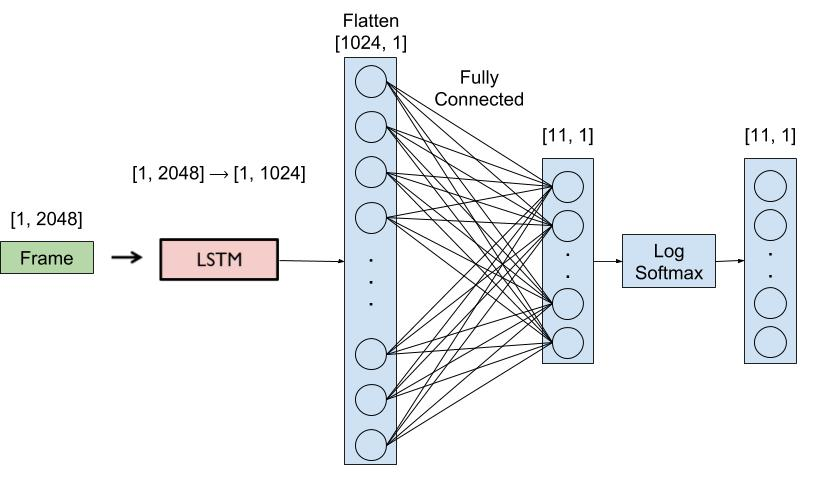
\includegraphics[width=\textwidth]{week10-lstmclassification-lamem-v1.jpg}
\caption{LSTM Classification for LaMem v1.}
\end{figure}

Because I only trained my network on this dataset for 20 epochs so the loss value was nearly remain from the initialization. In the other hand, the accuracy was too turbulent also. So I guess that my network architecture had some defects so it was not stable at all. The maximum accuracy was \textbf{\emph{31\%}} and the minimum value of loss was \textbf{\emph{16.26}}. These figures below described the loss valueand accuracy over epoch.

It took me around \textbf{\emph{1.8 hours}} to train 20 epochs (\textbf{\emph{5.5 mins}} per epoch).

\begin{figure}[!ht]
\centering
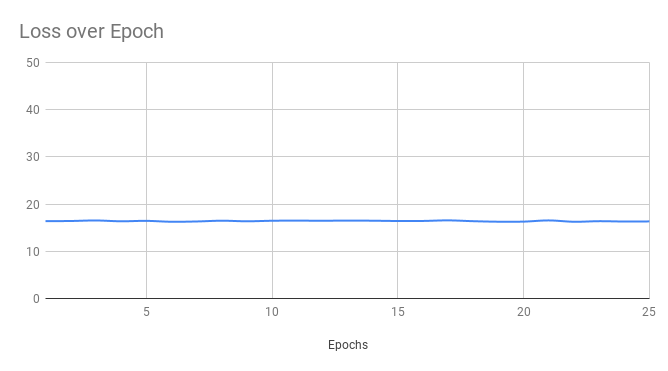
\includegraphics[width=\textwidth]{week10-lamem-v1-loss.png}
\caption{Loss over Epoch.}
\end{figure}

\begin{figure}[!ht]
\centering
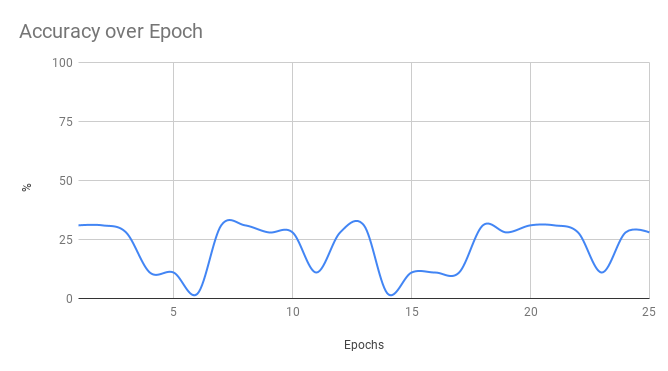
\includegraphics[width=\textwidth]{week10-lamem-v1-accuracy.png}
\caption{Accuracy over Epoch.}
\end{figure}